% This is based on "sig-alternate.tex" V1.9 April 2009
% This file should be compiled with V2.4 of "sig-alternate.cls" April 2009
%
\documentclass{report}

\usepackage[english]{babel}
\usepackage{graphicx}
\usepackage{tabularx}
\usepackage{subfigure}
\usepackage{enumitem}
\usepackage{url}


\usepackage{color}
\definecolor{orange}{rgb}{1,0.5,0}
\definecolor{lightgray}{rgb}{.9,.9,.9}
\definecolor{java_keyword}{rgb}{0.37, 0.08, 0.25}
\definecolor{java_string}{rgb}{0.06, 0.10, 0.98}
\definecolor{java_comment}{rgb}{0.12, 0.38, 0.18}
\definecolor{java_doc}{rgb}{0.25,0.35,0.75}

% code listings

\usepackage{listings}
\lstloadlanguages{Java}
\lstset{
	language=Java,
	basicstyle=\scriptsize\ttfamily,
	backgroundcolor=\color{lightgray},
	keywordstyle=\color{java_keyword}\bfseries,
	stringstyle=\color{java_string},
	commentstyle=\color{java_comment},
	morecomment=[s][\color{java_doc}]{/**}{*/},
	tabsize=2,
	showtabs=false,
	extendedchars=true,
	showstringspaces=false,
	showspaces=false,
	breaklines=true,
	numbers=left,
	numberstyle=\tiny,
	numbersep=6pt,
	xleftmargin=3pt,
	xrightmargin=3pt,
	framexleftmargin=3pt,
	framexrightmargin=3pt,
	captionpos=b
}

% Disable single lines at the start of a paragraph (Schusterjungen)

\clubpenalty = 10000

% Disable single lines at the end of a paragraph (Hurenkinder)

\widowpenalty = 10000
\displaywidowpenalty = 10000
 
% allows for colored, easy-to-find todos

\newcommand{\todo}[1]{\textsf{\textbf{\textcolor{orange}{[[#1]]}}}}

% consistent references: use these instead of \label and \ref

\newcommand{\lsec}[1]{\label{sec:#1}}
\newcommand{\lssec}[1]{\label{ssec:#1}}
\newcommand{\lfig}[1]{\label{fig:#1}}
\newcommand{\ltab}[1]{\label{tab:#1}}
\newcommand{\rsec}[1]{Section~\ref{sec:#1}}
\newcommand{\rssec}[1]{Section~\ref{ssec:#1}}
\newcommand{\rfig}[1]{Figure~\ref{fig:#1}}
\newcommand{\rtab}[1]{Table~\ref{tab:#1}}
\newcommand{\rlst}[1]{Listing~\ref{#1}}

% General information

\title{Project Title\\
\normalsize{Distributed Systems -- Project Proposal}}
\subtitle{subtitle}

% Use the \alignauthor commands to handle the names
% and affiliations for an 'aesthetic maximum' of six authors.

\numberofauthors{6} %  in this sample file, there are a *total*
% of EIGHT authors. SIX appear on the 'first-page' (for formatting
% reasons) and the remaining two appear in the \additionalauthors section.
%
\author{
% You can go ahead and credit any number of authors here,
% e.g. one 'row of three' or two rows (consisting of one row of three
% and a second row of one, two or three).
%
% The command \alignauthor (no curly braces needed) should
% precede each author name, affiliation/snail-mail address and
% e-mail address. Additionally, tag each line of
% affiliation/address with \affaddr, and tag the
% e-mail address with \email.
%
% 1st. author
\alignauthor \normalsize{Valentin Trifonov}\\
	\affaddr{\normalsize{ETH ID 13-941-679}}\\
	\email{\normalsize{vatrifon@student.ethz.ch}}
% 2nd. author
\alignauthor \normalsize{Simon Ringeisen}\\
	\affaddr{\normalsize{ETH ID 13-934-930}}\\
	\email{\normalsize{rsimon@student.ethz.ch}}
% 3rd. author
\alignauthor \normalsize{Jan Eberhardt}\\
	\affaddr{\normalsize{ETH ID 13-925-417}}\\
	\email{\normalsize{ebjan@student.ethz.ch}}
\and
% 4th. author
\alignauthor \normalsize{Caroline Creidenberg}\\
	\affaddr{\normalsize{ETH 15-907-421}}\\
	\email{\normalsize{ccreiden@student.ethz.ch}}
% 5th. author
\alignauthor \normalsize{Fabian Ulb}\\
	\affaddr{\normalsize{ETH ID 13-931-951}}\\
	\email{\normalsize{fabianu@student.ethz.ch}}
% 6th. author
\alignauthor \normalsize{Felix Wolf}\\
	\affaddr{\normalsize{ETH ID 13-927-983}}\\
	\email{\normalsize{fewolf@student.ethz.ch}}
}


\begin{document}

\maketitle

\begin{abstract}
In this document we are describing the initial planning of an Android app, its purpose is to serve as a quick and easy way for people in an emergency situation to call for help to people within their vicinity. The goal of the app is that the people in the surrounding area will be able to receive the emergency alarm through peer-to-peer or a server based system and respond to the emergency faster than any official emergency system would be able to. 
\end{abstract}

\section{Introduction}

Traditional emergency solutions tend to have one issue making them unsuitable for many modern emergency situations, that is the need for a longer conversation about the problem with an officer and the long response latency. In some situations, much faster help is needed.
We try to tackle this problem by providing an application which is very easy and fast to start, issuing an alert to people nearby informing them of the emergency as well as the location, and therefore enabling people helping people where needed, even in situations where an internet connection might not be available.

As good as this sounds, there are a number of challenges to solve for this, particularly concerning fast and reliable multicasts and consistency for proximity-based communication.

First of all, there is the problem of reliability - in an emergency situation, you want to have your alert reaching other people by any means possible. We try to tackle this by using multiple different means of communication and detection:
First of all, with a working internet connection, we will pursue a centralized approach, a firebase database to store the locations of people and a server to evaluate the location informations and send push notifications via Google Cloud Messaging (GCM) to notify people in the vicinity of the alert origin. Firebase is a scalable real-time database which was originally developed by an independant company and later got bought by google~\cite{firebase}. We choose this approach for scalability reasons. See section 2.1 for more details. This provides a large range as well as a reliable way of communication.

Secondly, without a working internet connection, we take a P2P approach. There is p2pkit~\cite{p2pkit}, a framework developed by a spinoff of the ETH, Ueppa, which is developed exactly for proximity-detection, and works even without an internet connection. Though this is a nice approach, the current development status of this framework might not be sufficient for our requirements. We started a first series of tests with modest results but we will evaluate our options here further. One consideration is to replace p2pkit with the Android Wifi-P2P framework~\cite{android_wifi_p2p} or use it as a supplement. In case we arrive at the decision that it is insufficient we will focus ourselves on the centralized approach and take P2P as a best effort offline approach. Consult Section 2.2. for more details.

The combination of these approaches should hence provide reliability on the edge what’s possible with currently available technology.

\section{System Overview}

It's important to remember that we have two app backends that essentially do the same thing. They can be thought of as two different channels to communicate. If one is not available, we will just try to use the other option and if both are available that is fine as well.

\subsection{Centralized approach}

As mentioned in section 1 the centralized approach uses a central server and a database. All clients, meaning all phones on whom our app is running, register by sending their ID to the App Engine Server~\cite{google_app_engine}. They get back a key, which they can use to write to the database and write their location into. This location doesn't need to be accurate, it just needs to be a rough approximation. Also this location must be updated from time to time, this could be every hour, twice a day or even only daily. This allows us to store a rough location estimation of all the clients. Now if one client needs help, he sends an alarm request to the server. This request also contains his/her exact current location. The server then goes through the database and finds clients that are somewhat in the near. This could be 10 km or 100 km or even more depending on the update interval of the locations. Then the server sends a push notification via Google Cloud Messaging (GCM) to the clients which are in this larger range. See~\cite{firebase_app_engine_tutorial} for Firebase with Google App Engine and~\cite{gcm_template} for GCM push notifications. Then the clients can decide whether the request is not too old (as GCM's may be delayed when the client was offline) and if the user who needs help is within a useful range. It then connects to the firebase and looks to see if someone who is closer to the person who needs help has already taken action. If not, the app starts an alarm. As soon as the user decides to help, the app starts putting his/her current location into the server. Like this, the other users can see, whether someone has already taken action or not. The alarm can be revoked by inserting a corresponding message into the firebase. 
\newline

\begin{figure}[h]
	\centering
    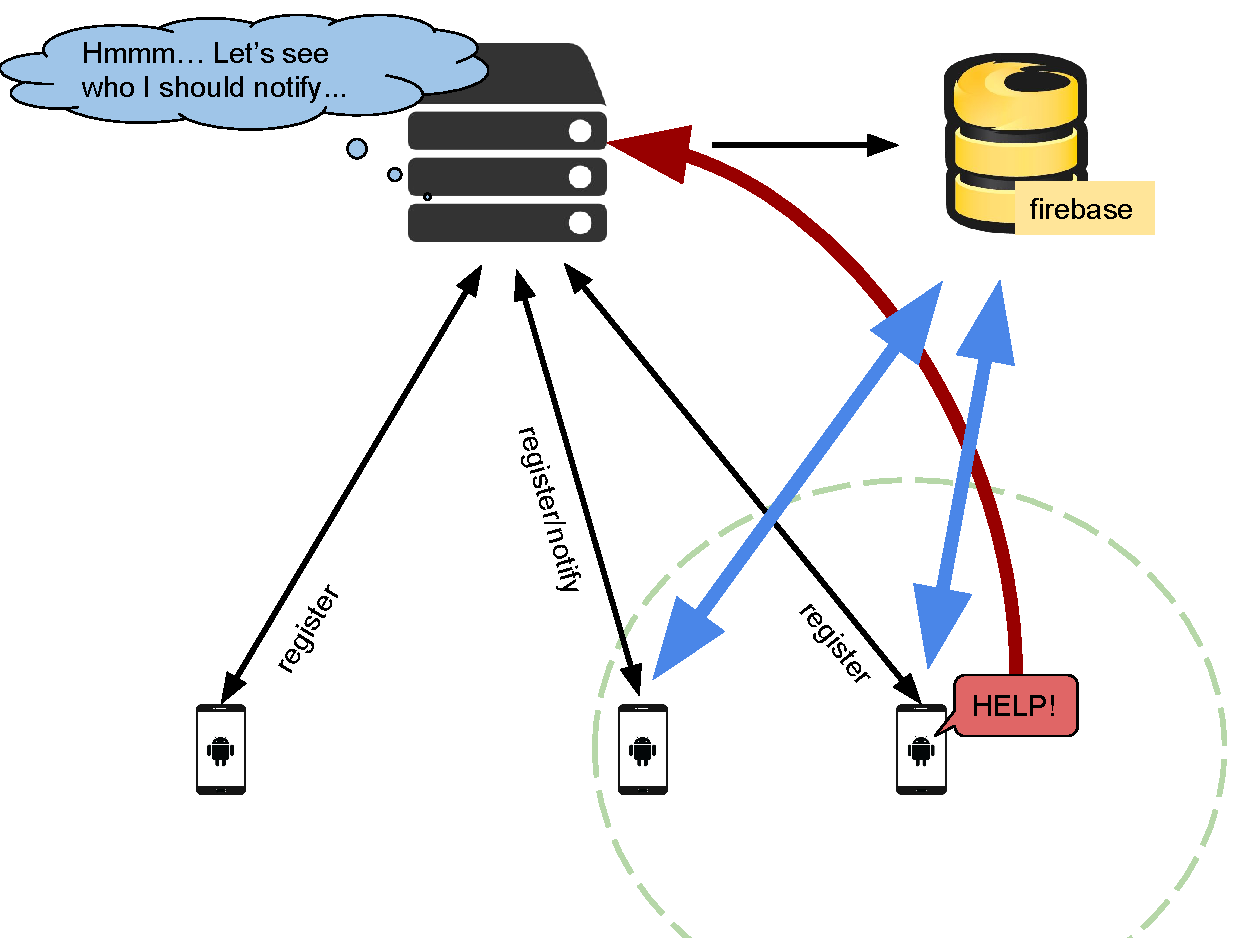
\includegraphics[width=\columnwidth]{server1.pdf}
    \lfig{server-structure}
    \vspace{-5mm} % use negative white space to fix too large gaps
	\caption{Server Structure}
\end{figure}

Why don't we use something like Google Nearby? 
With Google Nearby Messages one has a range restriction (approximately 30 meters)~\cite{nearby}. Since this is not enough for our purpose and we want to have flexible control of the range in which we want to alert people, we will build our own approach there. Therefore our system gets highly dynamic and would theoretically also work for any other kind of proximity based application.
Why do we use firebase and GCM and not our own simple server with, for example, simple MySQL database? We want our overall service to be reliable and highly scalable. We want to build a system which could theoretically be used by thousands of people. With firebase we are safe on the database side, because they claim they can handle millions of concurrent connections. Also we do not need to worry about security issues, encryption etc. We could theoretically always have an open connection to the firebase database directly from each client. This would require much energy according to~\cite{stackoverflow}. Therefore we rely on the GCM service there and send push notifications from our Google App Engine~\cite{google_app_engine} server via GCM to the client. Also with Google App Engine we do not need to worry about security and scalability issues. There are neat APIs for Android~\cite{firebase_java} and a REST Interface for the Server~\cite{firebase_rest}.

\subsection{Decentralized approach}

The Decentralized approach is currently based on the p2pkit. It can be divided in two parts, an active and a passive mode. In the passive mode each device has to keep track of the available peers in its vicinity. This gets implemented with a List, where discovered peers are inserted and lost peers are removed. Depending on which P2P technology we utilize, it could be that we can only deal with approximate times of actual existing peers.

\begin{figure}[h]
	\centering
    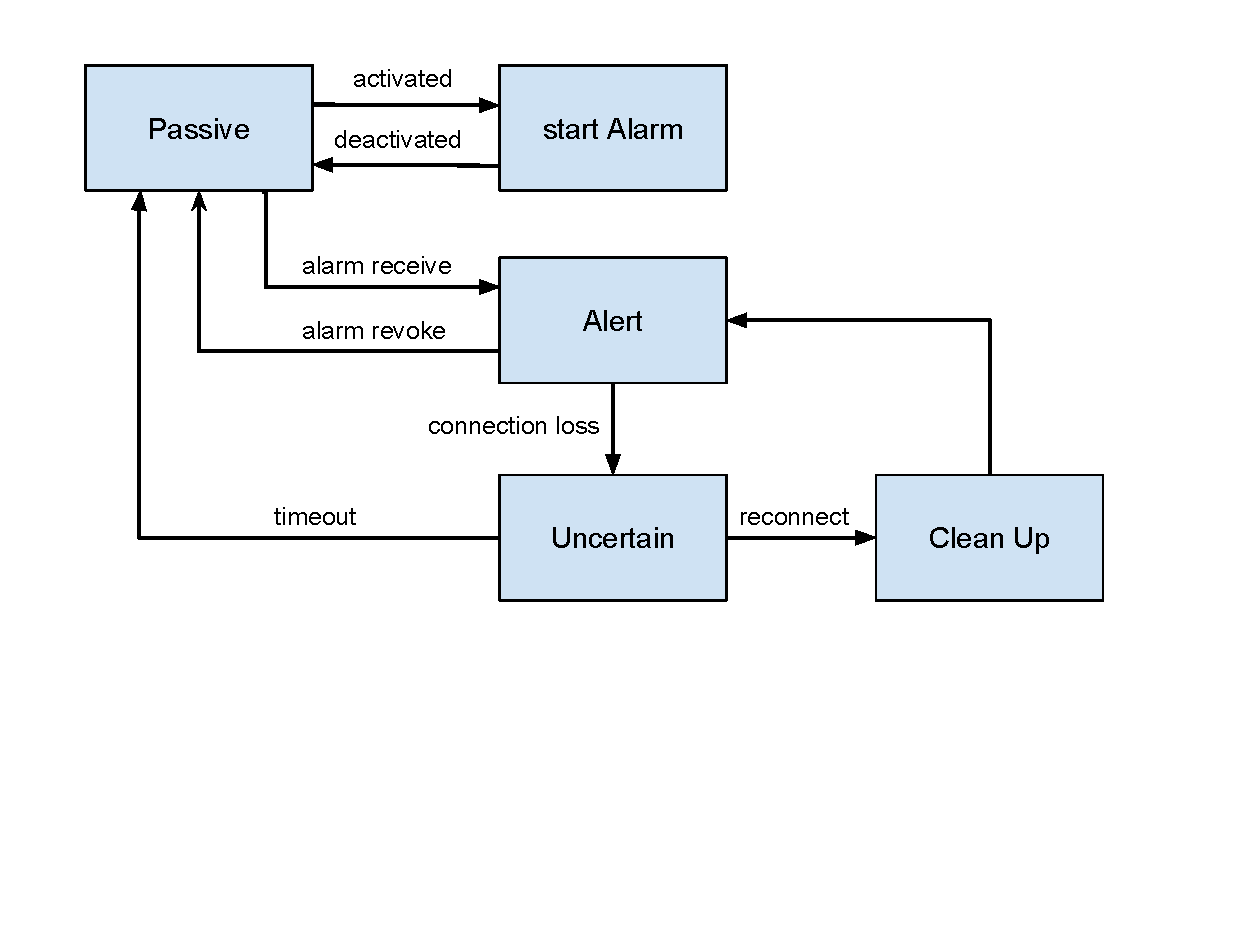
\includegraphics[width=\columnwidth]{peerControll.pdf}
    \lfig{peer-logic}
    \vspace{-5mm} % use negative white space to fix too large gaps
	\caption{Peer Logic}
\end{figure}

The App switches to active mode if an alarm is received or sent. If an alarm was sent, then the List of available peers is used to send them alarm messages. After an alarm was sent the user is given the possibility to revoke the alarm. The messages contain a source ID (UUID) and some information about the source location. If an alarm is received, the source id is stored until the alarm gets revoked. As long as the device has a connection to the device from which it got the source ID, it sends alarm messages to its available peers. To limit the number of resends, the devices keep track of the length of the path from the actual source to the device and if a certain threshold is reached it won't send any further messages. If a revocation with the source ID is received, it sends revocation messages to all its peers and goes back to passive mode. If the connection to the device from which it got the source ID is lost, it also won't send further alarm messages. If the connection with an involved device can be obtained, the device has to inquire if the alarm was not revoked, else the device will go back to passive mode after a certain timeout. In all states the user gets the possibility to return to passive mode.

\begin{figure}[h]
	\centering
    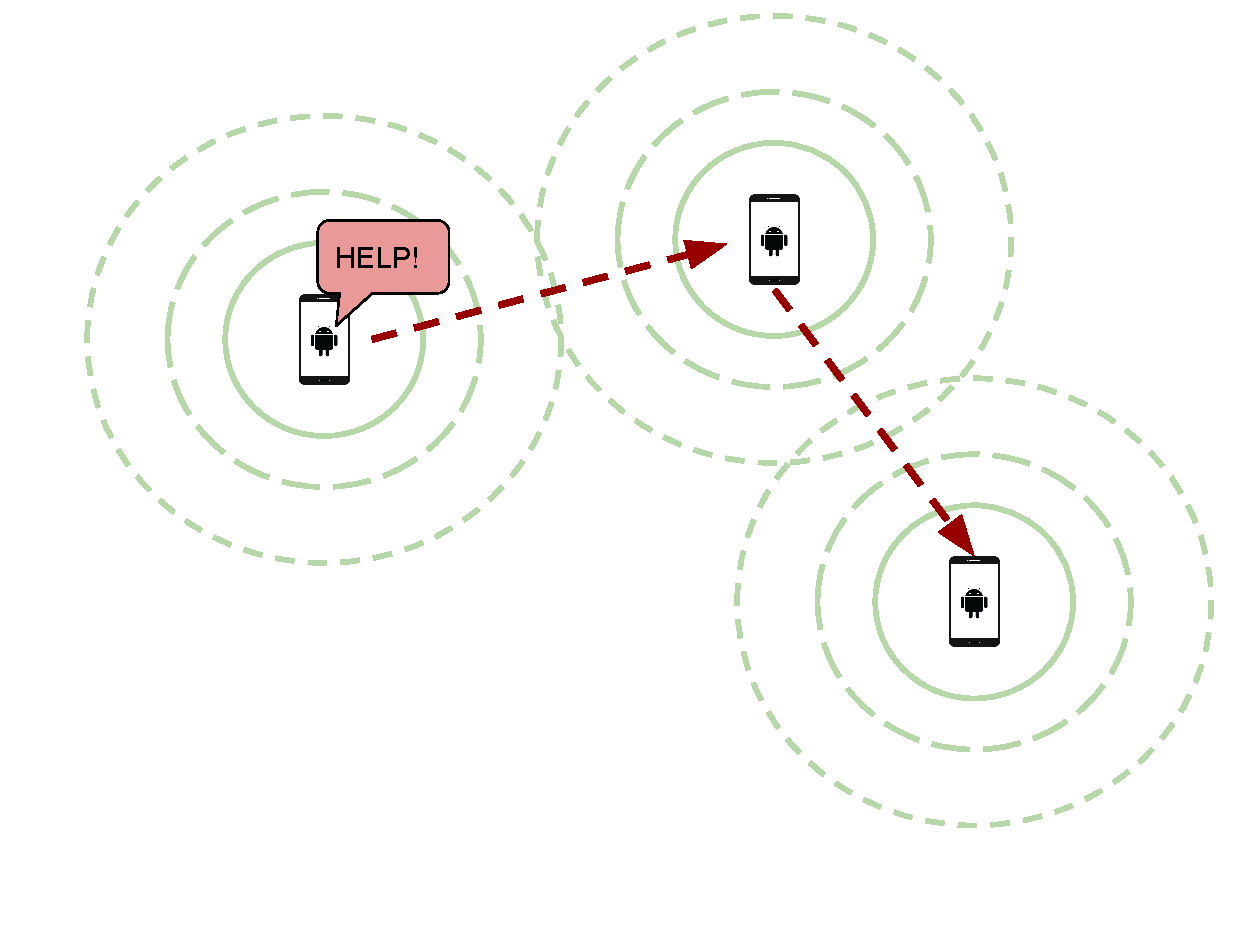
\includegraphics[width=\columnwidth]{P2P.pdf}
    \lfig{peer-connection}
    \vspace{-5mm} % use negative white space to fix too large gaps
	\caption{Peer Connection}
\end{figure}

Here the main challenge is to achieve consistency and fast communication between all devices with a reasonable battery usage. A first series of tests has shown certain issues in this domain, especially concerning the consistency.

\subsection{App Overview}
The picture below is a general overview of the system from an Android perspective and how we plan to implement the two separate channels.

\begin{figure}[h]
	\centering
    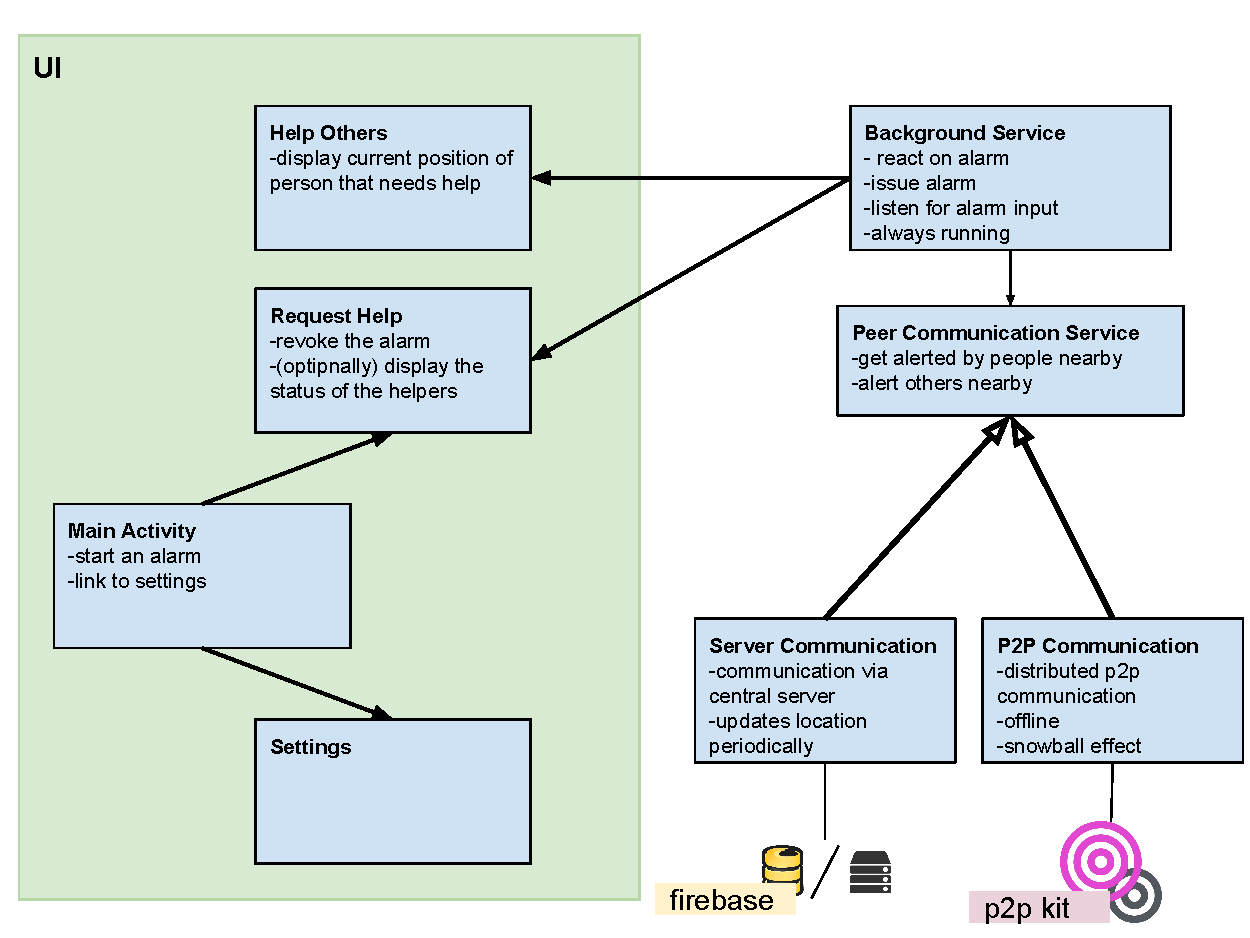
\includegraphics[width=\columnwidth]{AppOverview.pdf}
    \lfig{app-overview}
    \vspace{-5mm} % use negative white space to fix too large gaps
	\caption{App Overview}
\end{figure}

\subsection{UI}

The UI is pretty simple and straightforward. We have a Main Activity where you can start the alarm, turn the service as a whole either on or off (this means you won't receive alarms if it's off and you also will not be able to start an alarm) and a button to open the settings. The following  settings will be offered: the user can decide which button combination can trigger the alarm, turn off the online version and work with the p2p version only (this will only be implemented if the p2p communication will be sufficient) and enter a custom message which will be displayed to persons that get the alarm. If the user triggered the alarm he gets to a screen where he can abort or revoke said alarm and see the status of surrounding people, people on the way etc. (this is an optional feature). If somebody receives an alarm, there will be a standard android notification and by clicking on it, the user will get to a screen where he/she sees a map with his/her position and the location and message of the person in need. He/she is then able to either accept or dismiss the alarm depending on their ability to help or not.

\begin{figure}[h]
	\centering
    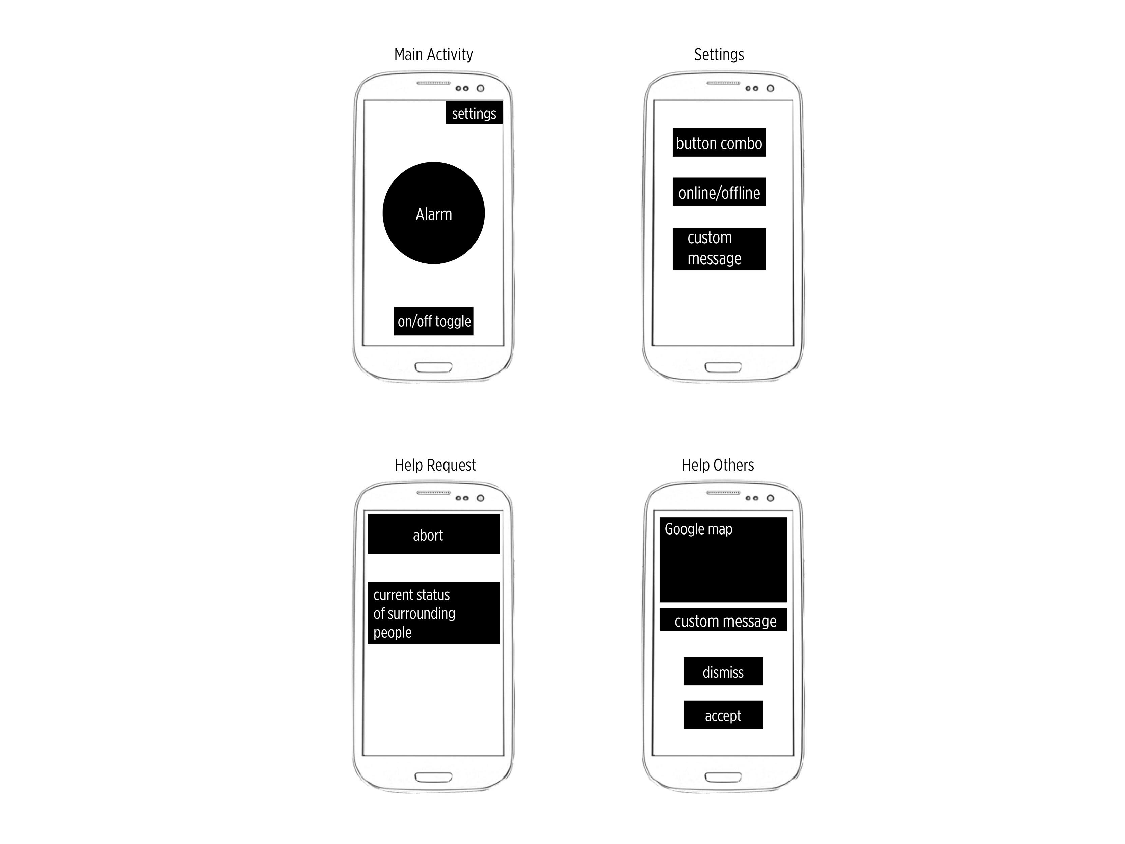
\includegraphics[width=\columnwidth]{Notruf.pdf}
    \lfig{app-ui}
    \vspace{-5mm} % use negative white space to fix too large gaps
	\caption{User Interface}
\end{figure}

\section{Requirements}
Because of a potential use of Bluetooth Low Energy we require minimum sdk 18. We will be testing our project with Nexus 5, LG G3 and Nexus 6. In the case that the p2pkit integration is successful, we will furthermore require that the p2pkit (P2P Services by Ueppa AG) is also installed on the device and that bluetooth and wifi are enabled, not necessarily connected, while the app is in use. The server implementation requires an internet connection and also the location service of android should be turned on. 
Libraries we will use:
\begin{enumerate}
	\item
	Google App Engine~\cite{google_app_engine}
	\item
	Google Cloud Endpoints~\cite{google_cloud_endpoints}
	\item
	Google Cloud Endpoints Android API~\cite{google_cloud_endpoints_android}
	\item
	Google Cloud Messaging~\cite{google_cloud_messaging}
	\item
	Google Cloud Messaging Android API~\cite{google_cloud_messaging_android}
	\item
	Firebase~\cite{firebase}
	\item
	Firebase Android API~\cite{firebase_java}
	\item
	Firebase token generator~\cite{firebase_token_generator}
	\item
	p2pkit~\cite{p2pkit}
	\item
	potentially Android Wifi P2P~\cite{android_wifi_p2p}
\end{enumerate}

\section{Work Packages}
Breakdown the work to subtasks to meet the project requirements.
Define and describe these tasks.

\newcommand{\wpitem}[2]{\item\textbf{#1}\\#2}
\newcommand{\wpgroup}[2]{
    \item\textbf{#1}
    \begin{enumerate}[label*=\arabic*.]
        #2
    \end{enumerate}
}
\begin{enumerate}[label*=\arabic*.]
    \wpgroup{GUI \& Activities}{
        \wpitem{implement basic GUI}{}
        \wpitem{Structure the project}{provide interfaces for the different work packages}
        \wpitem{(Optional) Alarm Feedback \& Helper Proximity}{Add a feature where the one needing help receives feedback about people on their way to him and their distance}
    }
    \wpgroup{P2P backend}{
        \wpitem{P2P Test Phase, Basic Functionality}{
            test if the p2pkit is applicable for our needs (in terms of speed and reliability).
            If it is not, we will not pursue this option further
        }
        \wpitem{Discovery Logic}{implement discovering nearby people, keep track of peers in your vicinity}
        \wpitem{Alarm \& Revocation Logic (Snowball effect, Broadcast)}{implement sending and revoking alarms to nearby people and reacting to these events}
    }
    \wpgroup{Centralized Backend - Client Side}{
        \wpitem{Database Setup (Firebase)}{integrate a firebase db into our app, periodically update user location in the database}
        \wpitem{GCM integration}{}
        \wpitem{Server Interface}{Communication to the server and reacting to push notifications (send current location, start alarm)}
        \wpitem{Alarm logic}{check if alarm is still valid and user is in a useful range, react to alarm if nobody else already did, handle reaction of user}
        \wpitem{(Optional) Alarm Feedback \& Helper Proximity}{Add a feature where the one needing help receives feedback about people on their way to him and their distance}
    }
    \wpgroup{Centralized Backend - Server Side}{
        \wpitem{Implement server and integrate firebase db}{}
        \wpitem{GCM integration}{}
        \wpitem{Alarm Logic}{react to user alarm events and find nearby people}
        \wpitem{(Optional) Alarm Feedback \& Helper Proximity}{Add a feature where the one needing help receives feedback about people on their way to him and their distance}
    }
    \wpgroup{Miscellaneous}{
        \wpitem{Alarm Activation Logic}{implement a listener which monitors button events for a special combination and then triggers the alarm}
        \wpitem{always-on Android background process \& IPC}{figure out how to have the background code running in a separate process and how to communicate to it from the activities}
        \wpitem{(Optional) consider ways on how we could reduce spam alerts}{}
    }

\end{enumerate}
 
\section{Milestones}
\begin{enumerate}[label*=\arabic*.]
    \item\textbf{Implement the basic building blocks - by 2.12.2015}\\
        Caroline: WP1.1, WP1.2\\
        Felix, Fabian: WP2.1, WP2.2, WP2.3\\
        Jan: WP3.1, WP3.3\\
        Valentin: WP3.2, WP3.4\\
        Jan and Valentin: WP5.2\\
        Simon: WP4.1, WP4.2, WP4.3\\
    \wpgroup{Code review - continuously}{
    	\wpitem{We review our code in pairs (Caroline/Simon, Felix/Fabian, Jan/Valentin)}{}
    }
    \wpitem{Put the basic building blocks together - by 8.12.2015}{}
    \wpgroup{Test, fix and optimize - until 18.12.2015}{
    	\wpitem{WP5.1 done by Caroline}{}
    }
    \wpgroup{Consider adding some of the optional stuff}{
    	\wpitem{WP1.3}{}
    	\wpitem{WP3.5}{}
    	\wpitem{WP4.4}{}
    	\wpitem{WP5.3}{}
    }
\end{enumerate}
% The following two commands are all you need in the
% initial runs of your .tex file to
% produce the bibliography for the citations in your paper.
\bibliographystyle{abbrv}
\bibliography{report}  % sigproc.bib is the name of the Bibliography in this case
% You must have a proper ".bib" file

%\balancecolumns % GM June 2007

\end{document}
